\subsection{Distributed approach}
\label{subsec:ex1distr}

\subsubsection{Model training}
\label{subsubsec:learneddist}

Once, enough data are collected through the simulator by using the optimal 
controller, it is possible to train a very simplified ``distributed network'' 
that takes as input an array containing the response values of the sensors – 
which can be either \texttt{prox\_values}, \texttt{prox\_comm} or 
\texttt{all\_sensors} – and produces as output an array containing one float 
that represents the speed of the wheels, which is assumed to be the same 
both right and left.

The dataset then contains a fixed number of simulation runs, each of these 
composed by a variable quantity of timesteps. It is important to notice that 
for this approach, unlike the one with communication, it is not necessary to 
keep the order of the sequence of timesteps, neither to know the exact 
number of agents in the simulation since the network input is the sensing 
associated to a single robot.

For this reason, the model is independent of the number of agents and 
consequently it is possible to prove its generalisation capacity, regardless 
the number of robots, by training the networks first on datasets each with a 
different but fixed value of $N$ and then on simulations composed by a 
variable $N$.
It is easy to show that although the value of $N$ changes the network 
structure does not, as it is sufficient during the input preprocessing to 
change the dimension of the input in such a way that all the tensors have a 
the same length, fixed at the maximum possible value of $N$, padding 
those tensors with a lower number of agents.

Thanks to these two assumptions, it is possible to shuffle the original 
dataset, based on the single run, in order to improve the generalisation on 
the samples, and then split the resulting collection into the train, the 
validation and the test sets, containing respectively $60$-$20$-$20\%$ of 
the data. 

The architecture of the network, displayed in Figure 
\ref{fig:singlenetdistributed1}, is straightforward: there are three linear 
layers each of size $\langle\mathtt{input\_size}, 10\rangle$,  $\langle 10, 
10\rangle$ and $\langle 10, 1\rangle$, where \texttt{input\_size} is the 
shape of the sensing, that can be $7$ or $14$.

\begin{figure}[htb]
	\centering
	\begin{subfigure}[h]{0.495\textwidth}
		\centering
		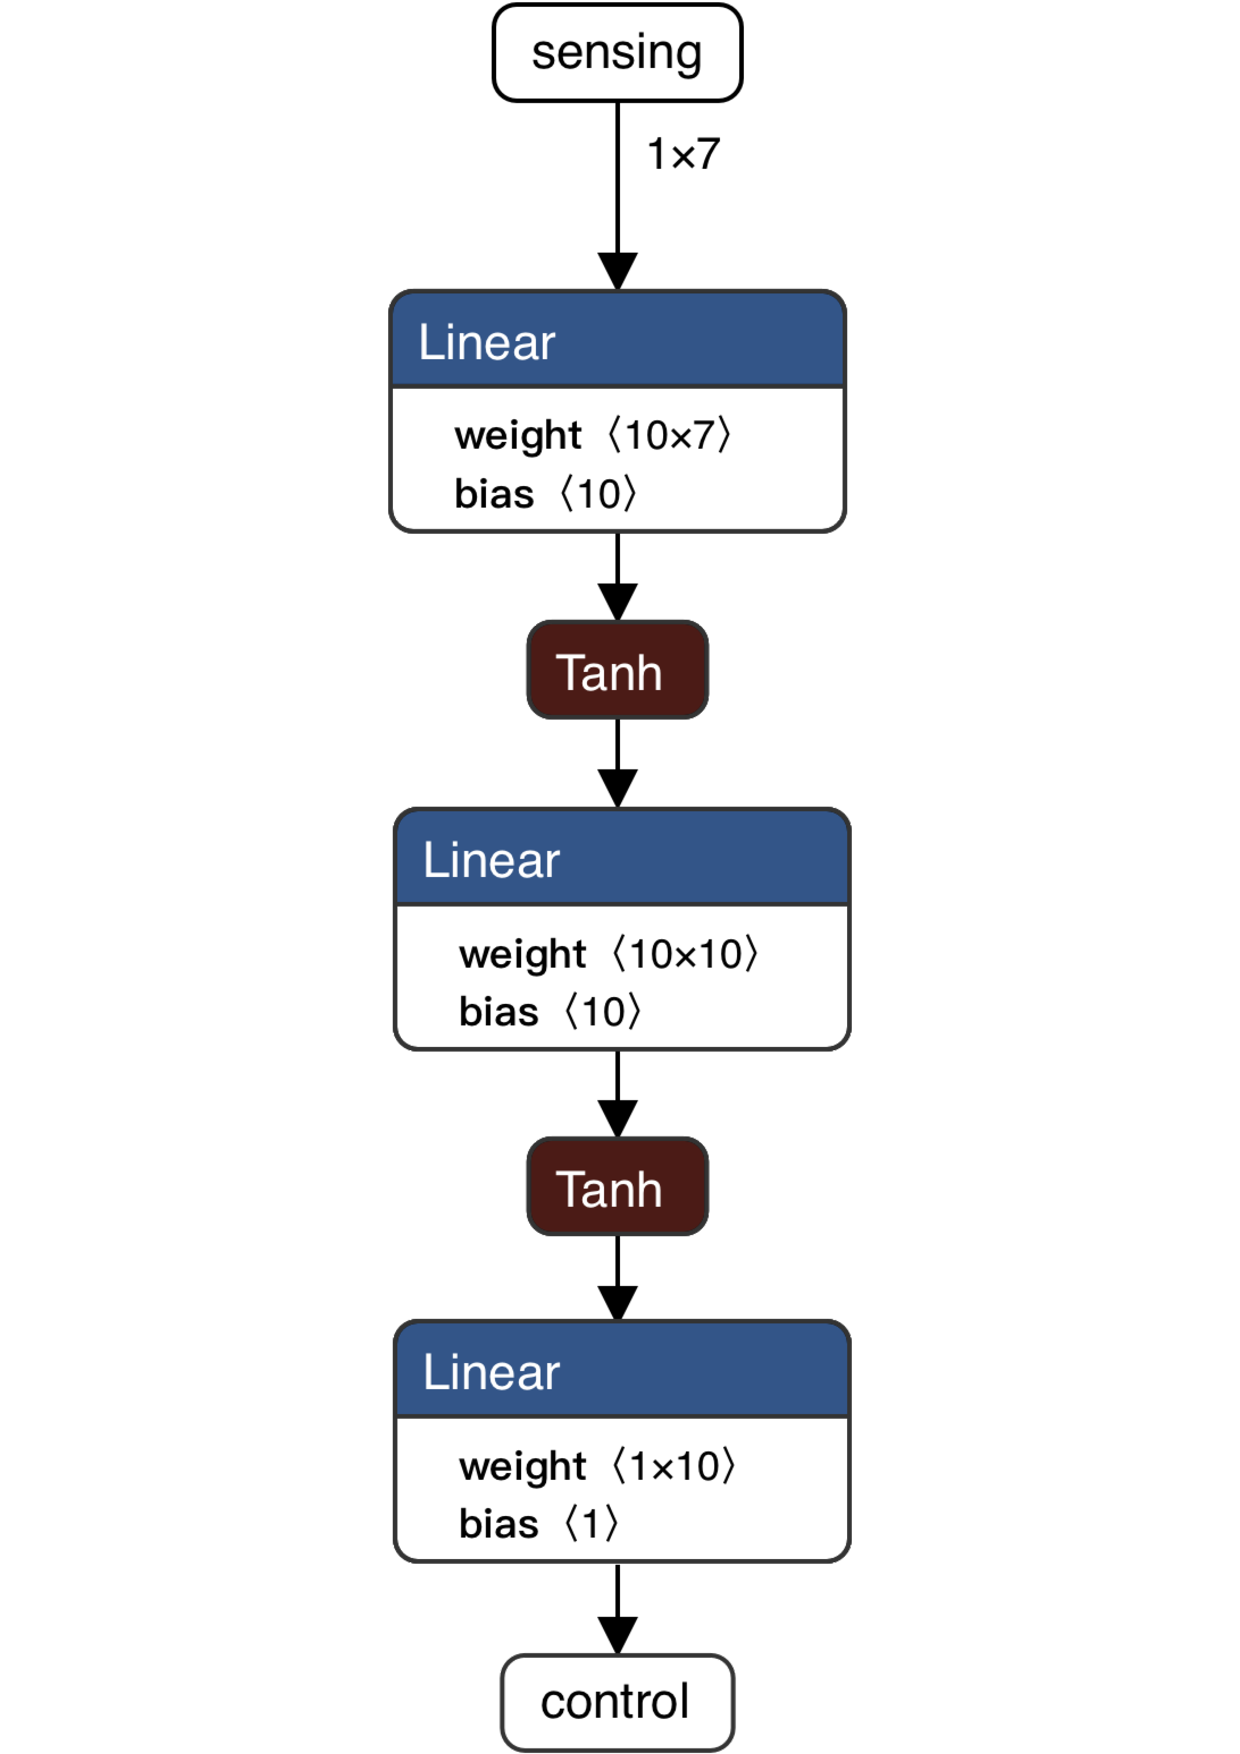
\includegraphics[width=.3\textwidth]{contents/images/task1distributed@4x}%
		\caption{Structure of a network with $7$ input sensing.}
		\label{fig:singlenet7distributed1}
	\end{subfigure}
	\hfill
	\begin{subfigure}[h]{0.495\textwidth}
		\centering
		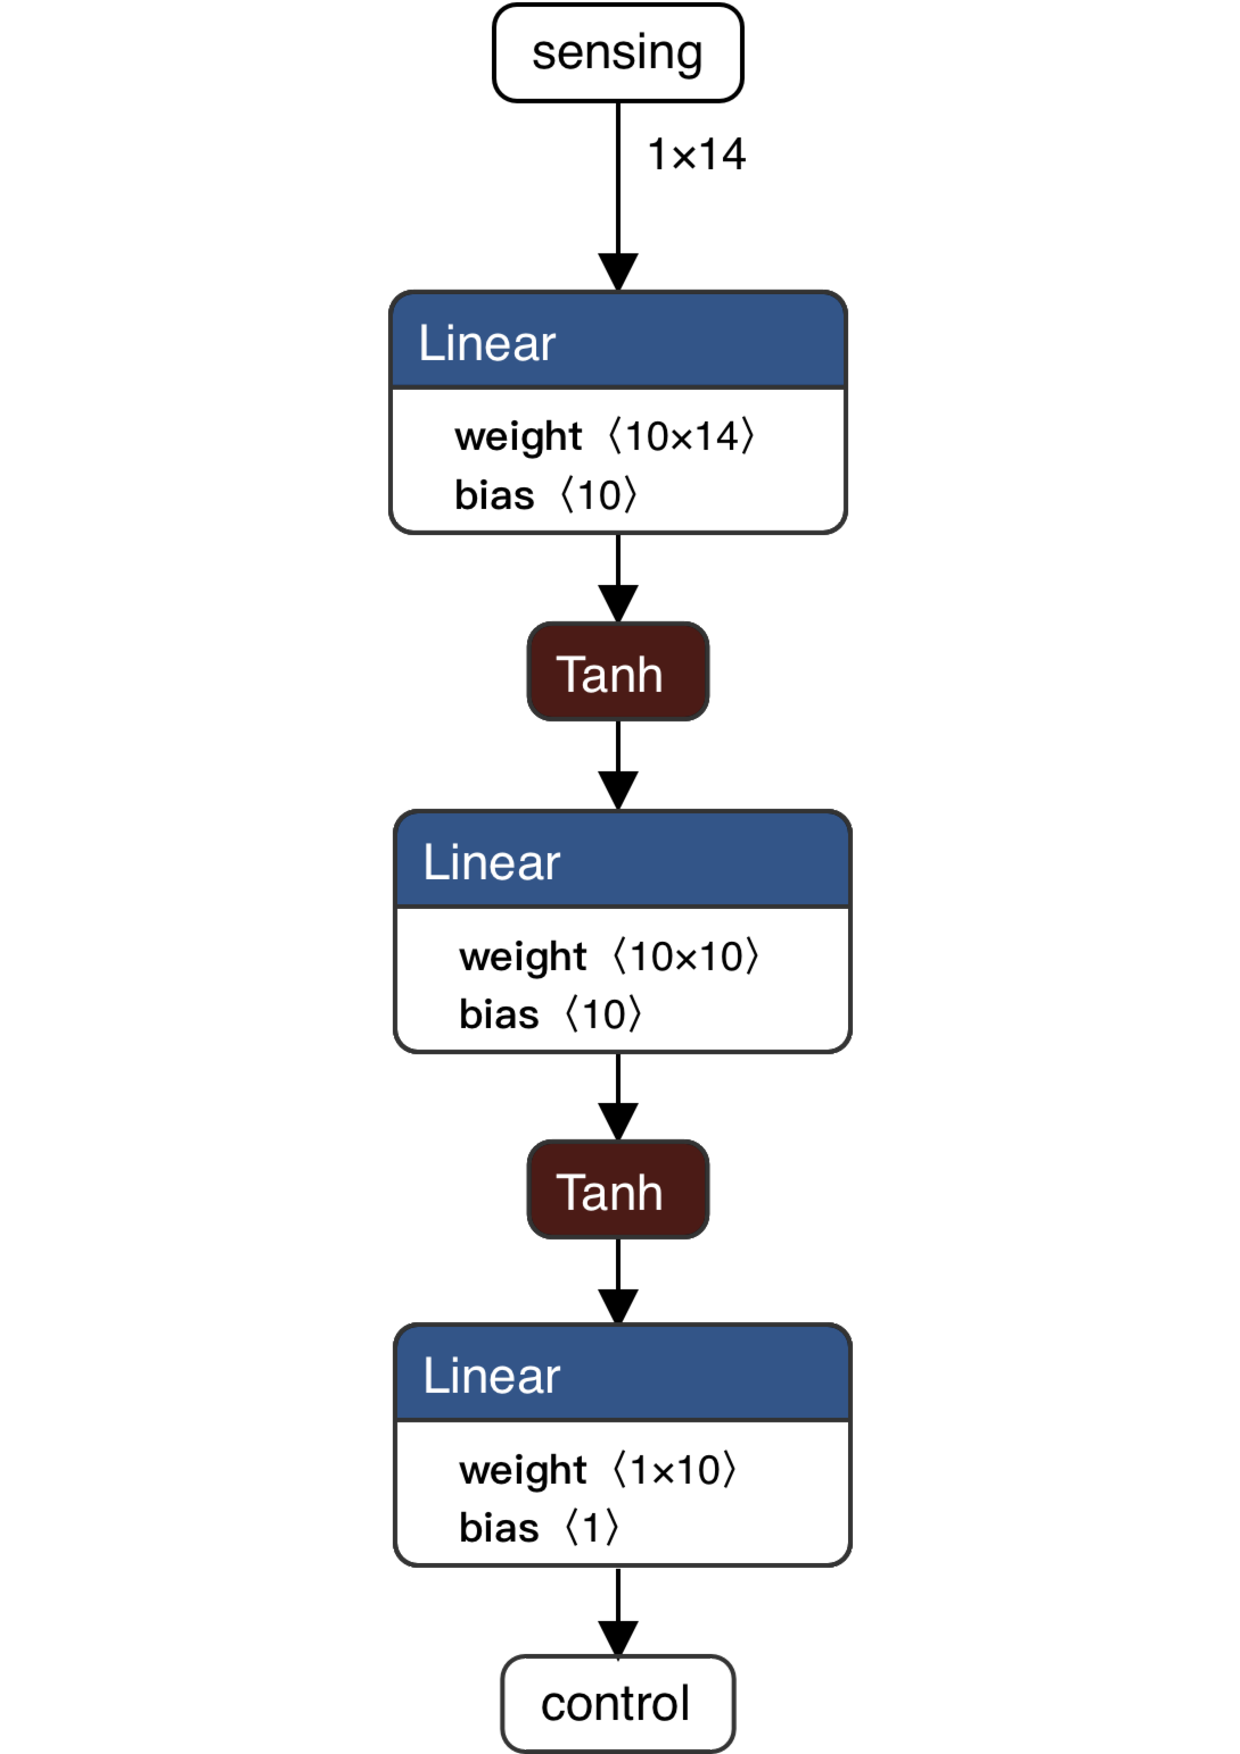
\includegraphics[width=.3\textwidth]{contents/images/task1distributed_all@4x}
		\caption{Structure of a network with $14$ input sensing.}
		\label{fig:singlenet14distributed1}
	\end{subfigure}
	\caption[Network architectures for the distributed approach.]{Visualisation of 
	the network architectures for the distributed approach.}
	\label{fig:singlenetdistributed1}
\end{figure}

To the first and second layer is applied a non-linear activation function, 
useful to make the model generalise. 
In particular, we chose the hyperbolic tangent (Tanh) 
\cite[see][]{kalman1992tanh}, a zero-centred function, shown in Figure 
\ref{fig:tanh}, whose range lies between $[-1, 1]$ and its output is given by

\begin{Equation}[H]
	\centering
	\begin{equation}
	f(x)= \frac{\sinh (x)}{\cosh (x)} = \bigg( \frac{e^x - e^{-x}}{e^x + 
		e^{-x}}\bigg)
	\end{equation}
	\caption{Hyperbolic Tangent Function (Tanh).}
	\label{eq:tanh}
\end{Equation}

This type of activation function is often used in deep learning and one of is 
advantages is that negative inputs are mapped to strongly negative values.

\begin{figure}[!htb]
	\centering
	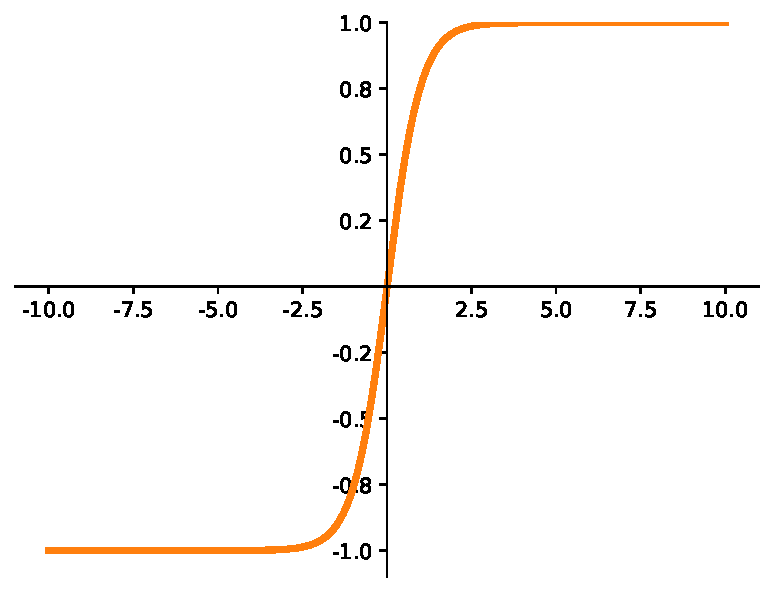
\includegraphics[width=.5\textwidth]{contents/images/tanh2}%
	\caption{Trend of the Tanh activation function.}
	\label{fig:tanh}
\end{figure}

%fixme citation
As optimiser we chose Adam, {an algorithm for first-order gradient-based 
optimisation of stochastic objective functions, based on adaptive estimates of 
lower-order moments}, \cite[see][]{kingma2014adam, 
loshchilov2017decoupled}, 
implemented in the \texttt{torch.optim} package, with a learning rate of $0.01$. 

Instead of computing the gradient descent on the entire dataset, the training set is 
split in mini-batches of size $100$ and an approximation of the gradient is 
produced, which makes the algorithm faster and at the same time, for sufficiently 
large numbers, the result is indistinguishable.

Gradient descent algorithms are susceptible to ``get stuck'' in local minima.
Mini-batches shuffle facilitate to avoid this problem by enabling the gradient to 
``bounce'' out of eventual local minimum, making it more variable by exploiting 
randomness, thereby helping convergence.

All the models are trained for $50$ epochs and evaluated using the \gls{mse} loss 
function, often used in regression problems. 
This criterion, implemented in the \texttt{torch.nn} package, measures the 
average of squared error between predictions and targets and learns to reduce it 
by penalising big errors in the model predictions.

\begin{Equation}[!htb]
	\centering
	\begin{equation}
	\mathtt{MSE} = \frac{\sum_{i=1}^n (y_i-\hat y_i)^2}{n}
	\end{equation}
	\caption{Mean Squared Error (\gls{mse}) loss function.}
	\label{eq:mse}
\end{Equation}
	

\subsubsection{Experiments}
\label{subsubsec:expdist}

The first group of experiments carried out, summarised in Table 
\ref{tab:modeln5dist}, examines the behaviour of the control learned in the case 
of the three different inputs, \texttt{prox\_values}, \texttt{prox\_comm} or 
\texttt{all\_sensors}, for a number of robots $N$ and an \texttt{avg\_gap} both 
fixed respectively at $5$ and the second chosen between $8$, $13$ and $24$.
\begin{figure}[H]
	\centering
	\begin{tabular}{llrr}
		\toprule
		\textbf{Model} \quad & \textbf{\texttt{network\_input}} & 
		\textbf{\texttt{input\_size}} &
		\textbf{\texttt{avg\_gap}} \\
		\midrule
		\texttt{net1} 				 & \texttt{prox\_values}	&  $  7$  &  $  8$  \\
		\texttt{net1b} 				& \texttt{prox\_values}	   &  $  7$  &  $13$ \\
		\texttt{net1c} 				& \texttt{prox\_values}	   &  $  7$  &  $24$  \\
		\texttt{net2} 				 & \texttt{prox\_comm}	  &  $  7$  &  $  8$  \\
		\texttt{net3} 				 & \texttt{prox\_comm}	  &  $  7$  &  $13$  \\
		\texttt{net4} 				 & \texttt{prox\_comm}	  &  $  7$  &  $24$  \\
		\texttt{net5} 				 & \texttt{all\_sensors}	  &  $14$  &  $  8$  \\
		\texttt{net6} 				 & \texttt{all\_sensors}	  &  $14$  &  $13$ 	\\
		\texttt{net7} 				 & \texttt{all\_sensors}	  &  $14$  &  $24$ 	\\
		\bottomrule
	\end{tabular}
	\captionof{table}{List of the experiments carried out with $5$ agents.}
	\label{tab:modeln5dist}
\end{figure}

First of all we start by showing in Figure \ref{fig:distloss} an overview of the 
models performance in terms of train and validation losses. 
\begin{figure}[!htb]
	\centering
	\includegraphics[width=.8\textwidth]{contents/images/task1/loss-distributed-all@x10}%
	\caption{Comparison of the losses of the models carried out with $5$ agents.}
	\label{fig:distloss}
\end{figure}

It is immediately evident that in case of \texttt{prox\_values} inputs the 
experiment performed with an \texttt{avg\_gap} of $24$ is not 
%FIXME synonim
significant/meaningful since this value exceeds the maximal range of the sensor.
In fact, from this analysis we generally expect a more stable behaviour using both 
types of input together, i.e. \texttt{all\_sensors}. 

For this reason, we start by exploring the results of the experiment obtained 
using 
the \texttt{prox\_values} readings alone as input of the network, continuing the 
with \texttt{prox\_comm} and concluding with \texttt{all\_sensors}.

The performance of \texttt{net1} are shown in the following images. In particular, 
we first visualise in Figure \ref{fig:net1r2} a comparison of the \gls{r2}, or 
coefficient of determination, of the manual and the learned controllers, on the 
validation set.
This score function evidences how well the regression predictions approximate 
the real data points (groundtruth). Since a model that perfectly predicts the data 
has a score of $1$, we assume that a higher score corresponds to a model that 
performs better.
\begin{figure}[!htb]
	\centering
	\begin{subfigure}[h]{0.49\textwidth}
		\centering
		\includegraphics[width=\textwidth]{contents/images/distr-net1/regression-manualvsomniscient}%
		%\caption{Expert controller output velocity.}
	\end{subfigure}
	\hfill
	\begin{subfigure}[h]{0.49\textwidth}
		\centering
		\includegraphics[width=\textwidth]{contents/images/distr-net1/regression-net1-vs-omniscient}
		%\caption{Distributed controller output velocity.}
	\end{subfigure}

	\caption[Evaluation of the \gls{r2} coefficient of \texttt{net1} .]{Comparison of 
	the \gls{r2} coefficient of the manual and the controller learned from 
	\texttt{net1} with respect to the omniscient one.}
	\label{fig:net1r2}
\end{figure}

From these figures we expect that the robots' behaviour using the learned 
controller instead of the manual one is a bit better, even if far from the 
omniscient 
controller.

In Figure \ref{fig:net1traj} we show first a comparison of the expert and the 
learned trajectories, and then between the manual and the learned ones. In 
particular, on the y-axis is visualised the position of each agent over time, while 
on the x-axis the simulation timesteps. It is important to notice that the plots 
summarise all the runs: at each timestep, the position of each agent is presented 
as an average over all the simulation runs, and in addition is  shown this average 
minus and plus the standard deviation.
\begin{figure}[!htb]
	\centering
	\begin{subfigure}[h]{0.49\textwidth}
		\centering
		\includegraphics[width=\textwidth]{contents/images/distr-net1/position-overtime-omniscient}%
		\caption{Expert controller trajectories.}
	\end{subfigure}
	\hfill
	\begin{subfigure}[h]{0.49\textwidth}
		\centering
		\includegraphics[width=\textwidth]{contents/images/distr-net1/position-overtime-distributed}
		\caption{Distributed controller trajectories.}
	\end{subfigure}
	\hspace*{\fill}%          % empty line absolutely necessary!
	
	\vspace*{8pt}%  
	
	\hspace*{\fill}%  
	\begin{subfigure}[h]{0.49\textwidth}
		\centering
		\includegraphics[width=\textwidth]{contents/images/distr-net1/position-overtime-manual}%
		\caption{Manual controller trajectories.}
	\end{subfigure}
	\hfill
	\begin{subfigure}[h]{0.49\textwidth}
		\centering
		\includegraphics[width=\textwidth]{contents/images/distr-net1/position-overtime-distributed}
		\caption{Distributed controller trajectories.}
	\end{subfigure}
	\caption[Evaluation of the trajectories learned by \texttt{net1}.]{Comparison 
		of trajectories generated using three controllers: the expert, the manual and 
		the one learned from \texttt{net1}.}
	\label{fig:net1traj}
\end{figure}

The robots convergence to the target using the omniscient controller is much 
faster than that with the manual or the learned one.
In particular, the learned trajectories, even if converge to the correct 
configuration they require a higher number of timesteps compared to the two 
others controllers. 

\begin{figure}[!htb]
	\centering
	\begin{subfigure}[h]{0.3\textwidth}
		\centering
		\includegraphics[width=\textwidth]{contents/images/distr-net1/control-overtime-omniscient}%
		\caption{Expert controller.}
	\end{subfigure}
	\hfill
	\begin{subfigure}[h]{0.3\textwidth}
		\centering
		\includegraphics[width=\textwidth]{contents/images/distr-net1/control-overtime-manual}%
		\caption{Manual controller.}
	\end{subfigure}
	\hfill
	\begin{subfigure}[h]{0.3\textwidth}
		\centering
		\includegraphics[width=\textwidth]{contents/images/distr-net1/control-overtime-distributed}
		\caption{Distributed controller.}
	\end{subfigure}
	\caption[Evaluation of the control learned by \texttt{net1}.]{Comparison 
		of output control generated using three controllers: the expert, the manual 
		and the one learned from \texttt{net1}.}
	\label{fig:net1control}
\end{figure}

In fact, analysing in Figure \ref{fig:net1control} the evolution of the control over 
time, it is possible to note that the omniscient and the manual controllers in the 
first timesteps have a higher speed than that predicted by the network. After 
about $15$ timesteps they both reach the target, with a certain tolerance, 
maintaining then the speed constant at $0$. Instead, the distributed controller 
decreases the speed of the agents as the timesteps pass, reaching zero speed but 
with a certain variance.

A couple of useful plots are shown below. In Figure \ref{fig:net1responsesensors} 
is visualised the response of the learned controller as the input sensing changes. 
\begin{figure}[!htb]
	\centering
	\begin{subfigure}[h]{0.49\textwidth}
		\centering
		\includegraphics[width=\textwidth]{contents/images/distr-net1/response-net1-front}%
		%\caption{response-net1-net([0, 0, x, 0, 0, 0, 0]).}
	\end{subfigure}
	\hfill
	\begin{subfigure}[h]{0.49\textwidth}
		\centering
		\includegraphics[width=\textwidth]{contents/images/distr-net1/response-net1-rear}
		%\caption{response-net1-net([0, 0, 0, 0, 0, x, x]).}
	\end{subfigure}
	\caption[Response of \texttt{net1} by varying the input sensing.]{Response of 
		\texttt{net1} by varying the input sensing.}
	\label{fig:net1responsesensors}
\end{figure}

In particular we analyse two cases. The first one shows the control predicted by 
the network when the robot sees nothing behind but only in front, more 
specifically when the given input is  $([0, 0, x, 0, 0, 0, 0])$, with $x$ varying in the 
range $[0, 4500]$.
The second shows the control predicted by the network when the robot instead 
sees nothing in front but only behind, more specifically when the given input is  
$([0, 0, 0, 0, 0,x , x])$, with $x$ varying in the range $[0, 4500]$.

The behaviour is almost as expected. When the robot sees nothing behind but 
something in front, the model returns a negative speed, since the robot has to 
move backwards. 
The absolute value of control increases as the proximity to the obstacle increases.
The same behaviour is obtained when the robot sees only behind but nothing in 
front. In this case the speed has the opposite sign.

Another informative plot, shown in Figure \ref{fig:net1responseposition}, displays 
the behaviour of a robot located between two that are already in their place.
\begin{figure}[!htb]
	\centering
	\includegraphics[width=.5\textwidth]{contents/images/distr-net1/response-varying_init_position-net1}%
	\caption{Response of \texttt{net1} by varying the initial position.}
	\label{fig:net1responseposition}
\end{figure}

It visualises the response of the learned controller to the variation of the distance 
between two stationary agents and a robot located halfway between them.
In particular, on the x-axis is visualised the position of the moving robot, while on 
the y-axis the output control, computed as an average over $100$ measures in 
which the pose of the agent $(x, y, \theta)$ is variated/varied by a certain epsilon 
uniformly distributed in the range $[-0.5\gls{cm}, 0.5\gls{cm}]$. In this way, the 
result obtained avoids the effects of noise that would be obtained on a single 
measurement and unrealistic artefacts in which the sensors are not continuous, 
compared to the pose, in simulation. In addition are also shown the bands that 
represent plus and minus standard deviation.

As expected, the output is a high positive value when the robot is close to an 
obstacle on the left, it decreases and reaches $0$ when the distance from right 
and left is equal, and finally becomes negative when there is an obstacle in front 
and not behind.

Finally, in Figure \ref{fig:net1distance} is presented another useful metric that 
measures the absolute distance of each robot from the target, visualised on the 
y-axis, over time. This value is averaged on all robots among all the simulation 
runs. The median value is shown as well as the interquartile and interdecile ranges.
\begin{figure}[!htb]
	\centering
	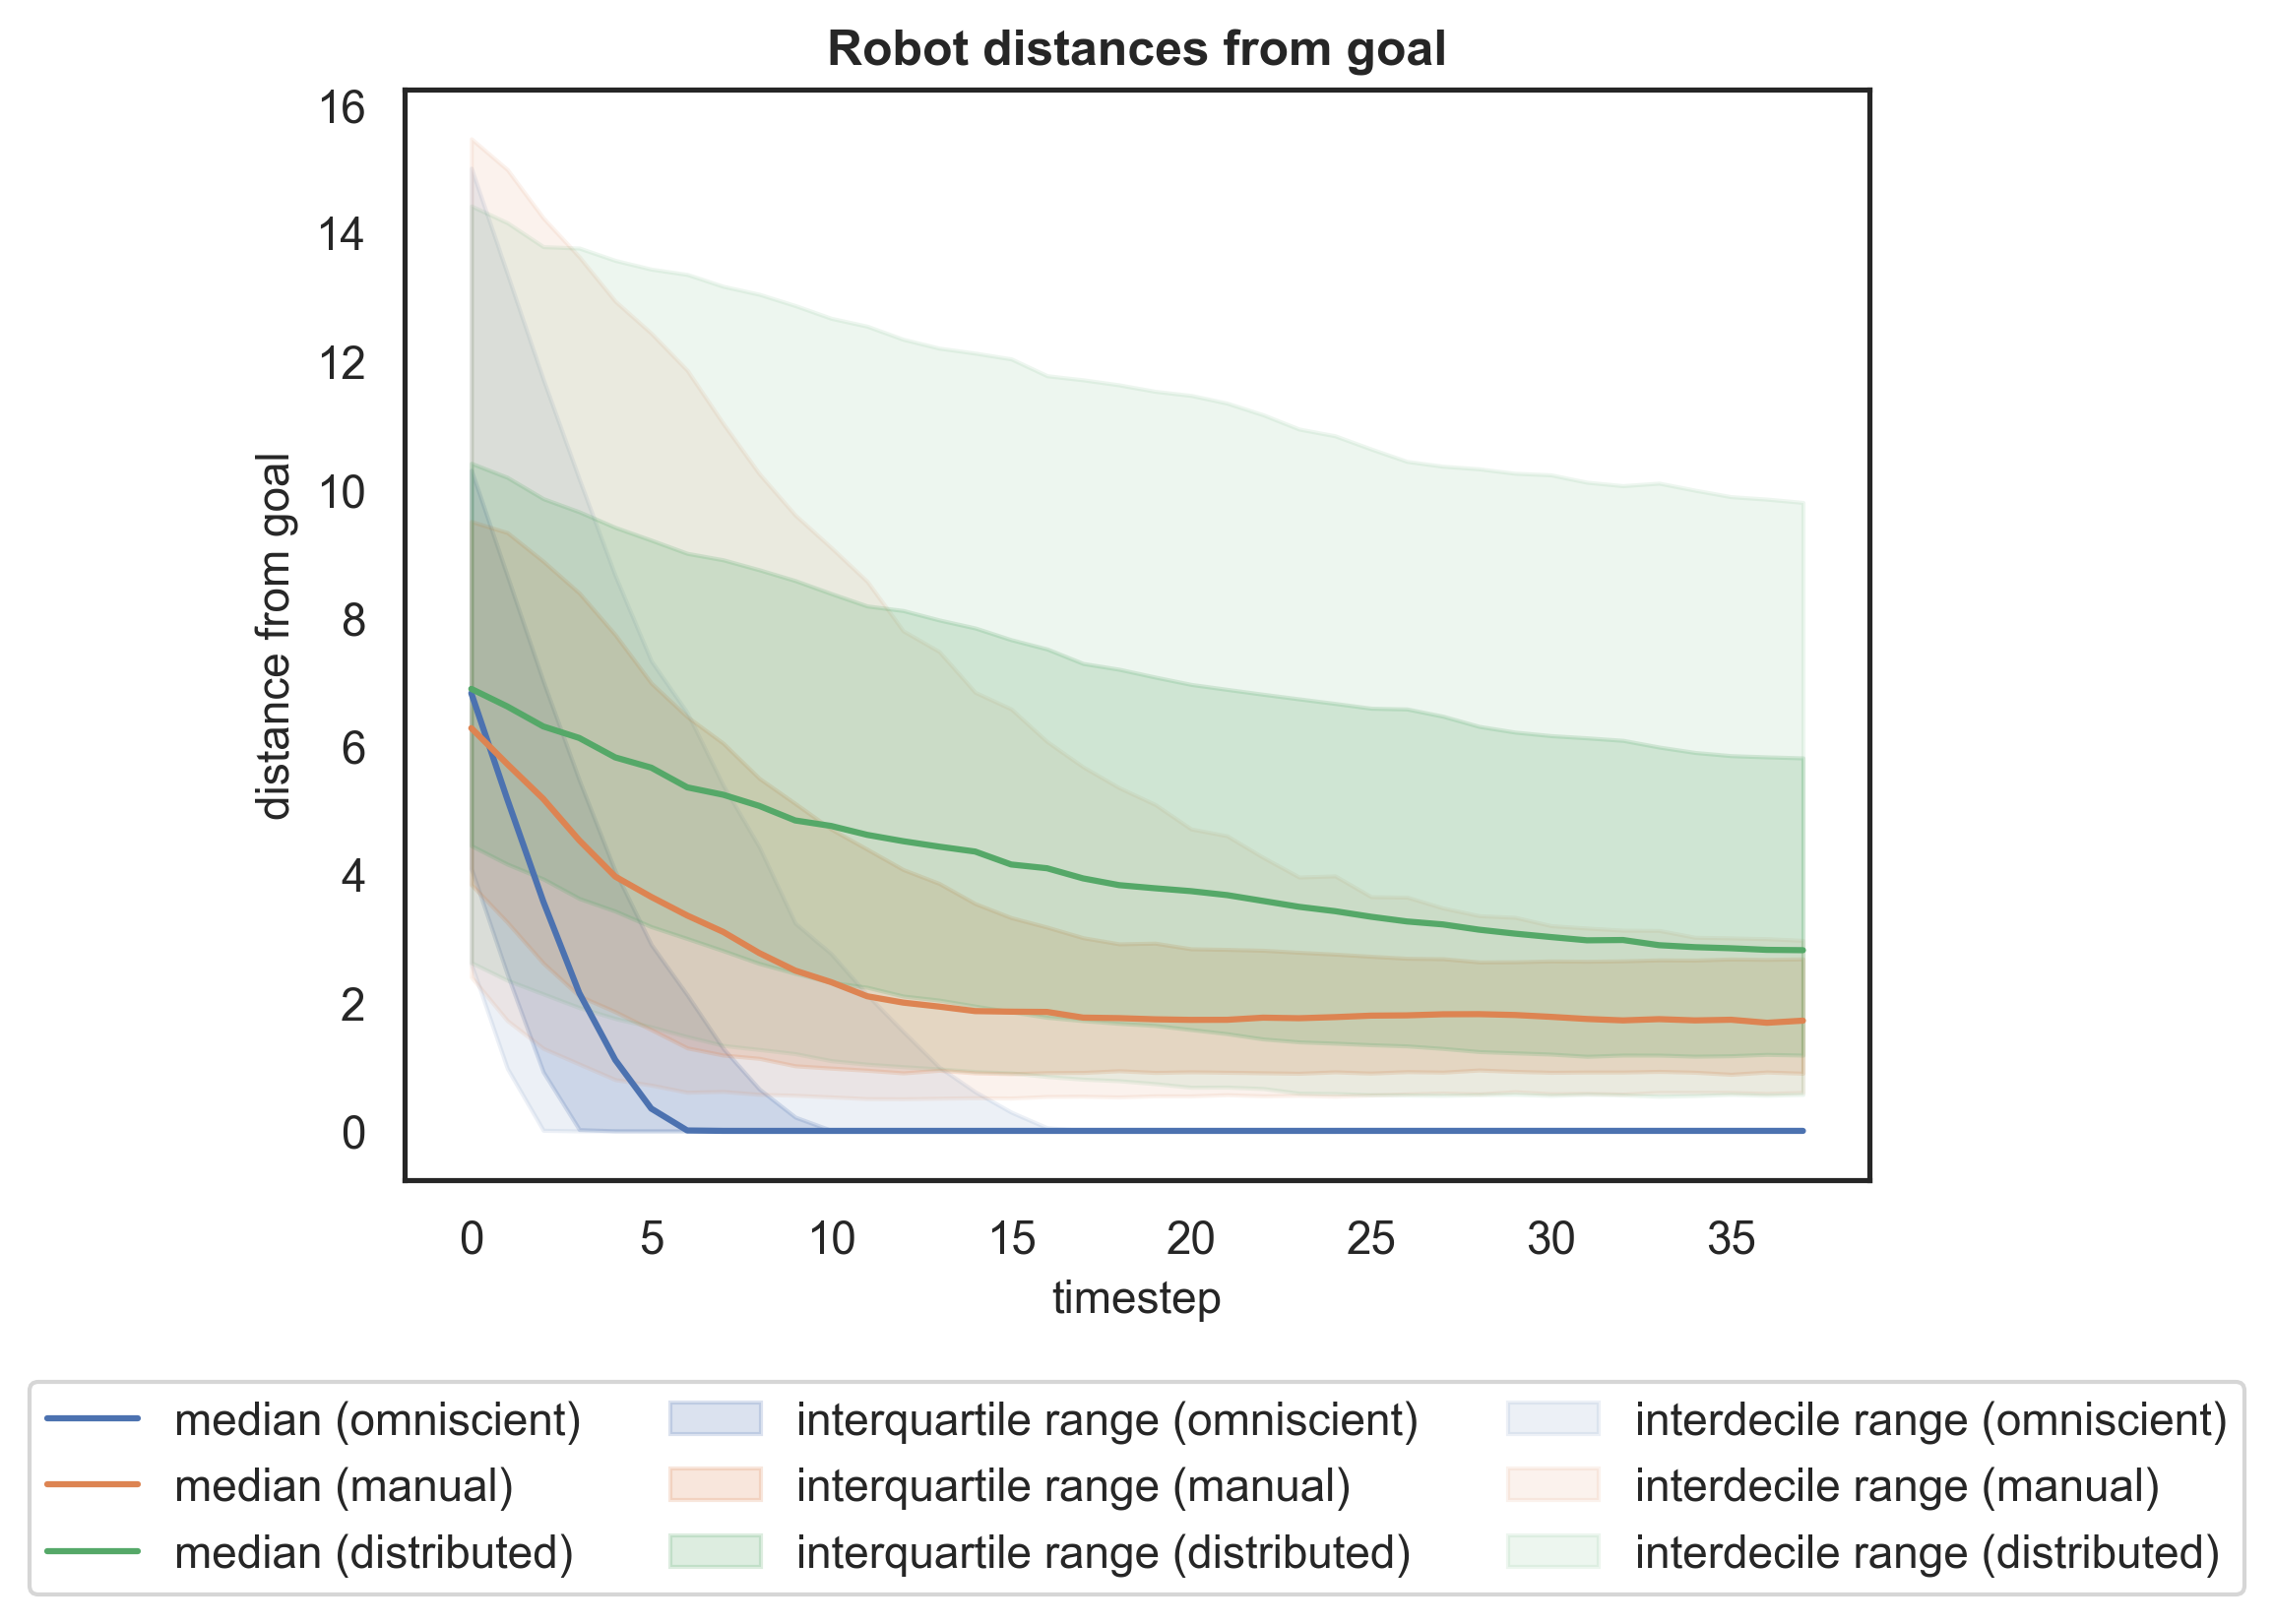
\includegraphics[width=.7\textwidth]{contents/images/distr-net1/distances-from-goal-compressed-distributed}%
	\caption{Comparison of the losses of the models carried out with $5$ agents.}
	\label{fig:net1distance}
\end{figure}

The plot shows that on average the distance from goal of the learned controller is 
is lower than the one obtained with the manual controller.

As mentioned before, in case of \texttt{prox\_values} inputs the 
experiment performed with an \texttt{avg\_gap} of $24$ is not meaningful since 
this value exceeds the maximal range of the sensor. Similarly, since $14$ is the 
maximum range, it is difficult to use this type of input when the \texttt{avg\_gap}  
is $13$, as shown by the losses in Figure \ref{fig:distlossprox_values}.

\begin{figure}[!htb]
	\centering
	\includegraphics[width=.75\textwidth]{contents/images/task1/loss-distributed-prox_values@x10}%
	\caption{Comparison of the losses of the models that use \texttt{prox\_values} 
	readings.}
	\label{fig:distlossprox_values}
\end{figure}

Following are shown the results of the experiments obtained using the 
\texttt{prox\_comm} readings. In Figure \ref{fig:distlossprox_comm}, are analysed 
the losses by varying the average gap. From a first observation the network seems 
to be able to work with all the gaps.

\begin{figure}[!htb]
	\centering
	\includegraphics[width=.75\textwidth]{contents/images/task1/loss-distributed-prox_comm@x10}%
	\caption{Comparison of the losses of the models that use \texttt{prox\_comm} 
	readings.}
	\label{fig:distlossprox_comm}
\end{figure}

Moving on to examine the \gls{r2} coefficients, instead are highlighted in Figure 
\ref{fig:net456r2}.

\begin{figure}[!htb]
	\begin{center}
		\begin{subfigure}[h]{0.45\textwidth}
			\includegraphics[width=\textwidth]{contents/images/distr-net4/regression-net4-vs-omniscient}%
			%\caption{Expert controller.}
		\end{subfigure}
		\hfill
		\begin{subfigure}[h]{0.45\textwidth}
			\includegraphics[width=\textwidth]{contents/images/distr-net5/regression-net5-vs-omniscient}%
			%\caption{\texttt{avg\_gap} 8 \gls{cm}.}
		\end{subfigure}
	\end{center}
	%\hspace*{\fill}%          % empty line absolutely necessary!
	%\vspace*{1pt}%  
	%\hspace*{\fill}%  
	\begin{center}
		\begin{subfigure}[h]{0.45\textwidth}
			\includegraphics[width=\textwidth]{contents/images/distr-net6/regression-net6-vs-omniscient}
			%\caption{Distributed controller.}
		\end{subfigure}
	\end{center}
	\caption[Comparison of the \gls{r2} coefficient for \texttt{prox\_comm} 
	readings.]{Comparison of the \gls{r2} coefficients of the models that use 
	\texttt{prox\_comm} readings.}
	\label{fig:net456r2}
\end{figure}

The coefficient obtained with \texttt{net6} is higher than the others, for this 
reason we expect a better behaviour of the model. Moreover, as shown in Figure 
\ref{fig:net6r2}, we expect that the robots’ behaviour using the learned controller 
instead of the manual one is better, even if far from the omniscient controller.

\begin{figure}[!htb]
	\centering
	\begin{subfigure}[h]{0.49\textwidth}
		\centering
		\includegraphics[width=\textwidth]{contents/images/distr-net6/regression-manualvsomniscient}%
		%\caption{Expert controller output velocity.}
	\end{subfigure}
	\hfill
	\begin{subfigure}[h]{0.49\textwidth}
		\centering
		\includegraphics[width=\textwidth]{contents/images/distr-net6/regression-net6-vs-omniscient}
		%\caption{Distributed controller output velocity.}
	\end{subfigure}
	
	\caption[Evaluation of the \gls{r2} coefficient of \texttt{net6} .]{Comparison of 
		the \gls{r2} coefficient of the manual and the controller learned from 
		\texttt{net6} with respect to the omniscient one.}
	\label{fig:net6r2}
\end{figure}

In Figure \ref{fig:net6traj} are shown the trajectories obtained employing the 
omniscient, the manual or the learned controller. As before, in the plots the robot 
positions are averaged over all the runs. 

\begin{figure}[!htb]
	\centering
	\begin{subfigure}[h]{0.49\textwidth}
		\centering
		\includegraphics[width=\textwidth]{contents/images/distr-net6/position-overtime-omniscient}%
		\caption{Expert controller trajectories.}
	\end{subfigure}
	\hfill
	\begin{subfigure}[h]{0.49\textwidth}
		\centering
		\includegraphics[width=\textwidth]{contents/images/distr-net6/position-overtime-distributed}
		\caption{Distributed controller trajectories.}
	\end{subfigure}
	\hspace*{\fill}%          % empty line absolutely necessary!
	
	\vspace*{8pt}%  
	
	\hspace*{\fill}%  
	\begin{subfigure}[h]{0.49\textwidth}
		\centering
		\includegraphics[width=\textwidth]{contents/images/distr-net6/position-overtime-manual}%
		\caption{Manual controller trajectories.}
	\end{subfigure}
	\hfill
	\begin{subfigure}[h]{0.49\textwidth}
		\centering
		\includegraphics[width=\textwidth]{contents/images/distr-net6/position-overtime-distributed}
		\caption{Distributed controller trajectories.}
	\end{subfigure}
	\caption[Evaluation of the trajectories learned by \texttt{net6}.]{Comparison 
		of trajectories generated using three controllers: the expert, the manual and 
		the one learned from \texttt{net6}.}
	\label{fig:net6traj}
\end{figure}

The robots convergence to the target using the omniscient controller is much 
faster than that with the manual or the learned one. In particular, the learned 
trajectories, even if converge to the correct configuration they require a higher 
number of timesteps compared to the two others controllers.

\begin{figure}[!htb]
	\centering
	\begin{subfigure}[h]{0.3\textwidth}
		\centering
		\includegraphics[width=\textwidth]{contents/images/distr-net6/control-overtime-omniscient}%
		\caption{Expert controller.}
	\end{subfigure}
	\hfill
	\begin{subfigure}[h]{0.3\textwidth}
		\centering
		\includegraphics[width=\textwidth]{contents/images/distr-net6/control-overtime-manual}%
		\caption{Manual controller.}
	\end{subfigure}
	\hfill
	\begin{subfigure}[h]{0.3\textwidth}
		\centering
		\includegraphics[width=\textwidth]{contents/images/distr-net6/control-overtime-distributed}
		\caption{Distributed controller.}
	\end{subfigure}
	\caption[Evaluation of the control learned by \texttt{net6}.]{Comparison 
		of output control generated using three controllers: the expert, the manual 
		and the one learned from \texttt{net6}.}
	\label{fig:net6control}
\end{figure}

